\chapter{Das Chlorophyll und sein Abbauprozess}

Jedes Jahr gehen weltweit schätzungsweise $10^{9}$ Tonnen an Chlorophyll scheinbar \textit{verloren}. Der Abbauprozess des Chlorophylls ist damit ob der markanten Farbveränderungen einer der visuell am meisten wahrgenommenen biochemischen Vorgänge und kann sogar aus dem All beobachtet werden \cite{ChlorophyllBreakdown}. Die schönen, bunten Farben des Laubs werden dabei jedoch nicht durch die Abbauprodukte des Chlorophylls (im Folgenden Chlorophyllkataboliten) hervorgerufen  \cite{DegradationChlorophyll}, da die Endprodukte des Chlorophyllabbaus farbblos sind \cite{ChlorophyllBreakdown}. Im Folgenden ist immer die Rede vom Abbauprozess in höheren Pflanzen, da gezeigt wurde, dass \gls{zB} marine Lebensformen das Chlorophyll auf einem anderen Wege abbauen und auch dementsprechend andere Endprodukte vorzufinden sind. \cite{ChlorophyllBreakdown}, \cite{ErsterKatabolit}, \cite{ChlorophyllCataboliteDifferent} Die Abbauprodukte fallen in die Kategorie der Phyllobiline und sind Anzeichen für Reifung, Seneszenz und den Zelltod. Der Abbauprozess wird im Rahmen eines Entgiftungsprozesses begannen. \cite{ChlorophyllKatabolitenalsZeichenReifung}

Die Struktur eines Chlorophyllkataboliten konnte erstmalig im Jahre 1991 aufgeklärt werden. Es handelte sich hierbei um einen Hv-\gls{NCC} der Gerste (\textit{Hordeum vulgare}) \cite{ErsterKatabolit}, das Endprodukt eines mehrstufigen Abbauprozesses. 

\begin{figure}[hbtp]
  \centering
  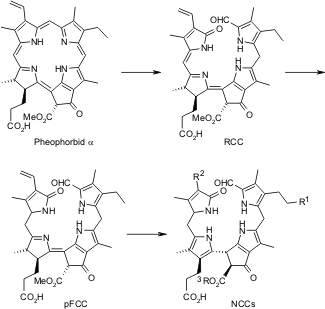
\includegraphics[scale=0.57]{figures/Kapitel2/VWA_Schema_Chlorophyllabbau.png}
  \caption[Abbauprozess des Chlorophylls, Quelle: http://www.organische-chemie.ch/chemie/2007nov/antioxidantien.shtm (Zugegriffen am: 05.11.2017)]{Der Abbauprozess des Chlorophylls in seneszenten Blättern}
  \label{fig:Chlorophyllabbau}
\end{figure}

\pagebreak
In den folgenden Jahren fand man heraus, dass das Chlorophyll zuerst in das Pheophorbid a umgewandelt wird. Im nächsten Schritt wird der Makrozyklus oxygenolytisch (an der Reaktion beteiligtes Enzym: Pheo \textit{a} Mono-oxygenase \cite{ChlorophyllCatabolitesEnzyme}) in der nördlichen \textit{meso} Position geöffnet, woraufhin ein \textit{Red Chlorophyll Catabolite} (RCC) entsteht. 
Über einen \textit{primary "flourescent" Chlorophyll Catabolite} (pFCC) entsteht durch eine nichtenzymatische Isomerisierung ein \gls{NCC}. Thermodynamische Triebkraft dieser Reaktion ist die Rearomatisierung von Ring D. \cite{FCCKatabolit}, \cite{ChlorophyllCatabolites} Die unterschiedlichen Arten von \gls{NCC}s ergeben sich durch Anlagerung der entsprechenden funktionellen Gruppen (\gls{zB} Zuckerring, Hydroxylgruppen, ...) an den pFCC. \cite{ChlorophyllCatabolites} In Abbildung \ref{fig:Chlorophyllabbau} sind die Positionen, an denen diese strukturellen Unterschiede auftreten können gekennzeichnet durch R\textsuperscript{1}, R\textsuperscript{2}, R\textsuperscript{3}.





